\chapter{tth eft}
\label{chap::tth_eft}
\chapterquote{The S\&P 500 is my favourite meme coin.}%
{Hannah Mehravari, after the Trump tariffs, Aprill 2025.}
With the $t\bar{t}H(b\bar{b})$ legacy analysis producing the most precise measurement of its kind to date, we believe it would be prevalent to re-interpret it with the SMEFT framework inorder to test for potential presence BSM effects. Using this analysis we can update the precision on the Wilson Coefficients (WC), which that dictate the strength of the SMEFT operators.
\section{Early Run-2 Results}
Before we proceed with the analysis, we should probably stop and take in the $t\bar{t}H$ EFT precision measurement landscape. Our main point of comparison for our results will be a early run-2 result from 2016 \cite{Maltoni:2016yxb}. The analysis in question used a combination of results from both the CMS and ATLAS detector. In order to break the degeneracy between the operators they use $H$, $H + j$ and $t\bar{t}H$ analyses: The $pp \to H$ measurements we are going to use are the following: in the diphoton channel we use \cite{ATLAS_2014,CMS_2014} at 8~TeV and \cite{CMS_2016_gg} at 13~TeV; in the $WW/ZZ/\tau\tau$ channels we use \cite{ATLAS_WW_2015,CMS_WW_2014,ATLAS_ZZ_2015,CMS_ZZ_2014,ATLAS_tau_2015,CMS_tau_2014}; measurements of $pp \to t\bar{t}H$ at 8~TeV in the diphoton channel are given in \cite{CMS_ttH_2014,ATLAS_ttH_2015_gamma}, while in the multilepton and $b\bar{b}$ channels we use \cite{CMS_ttH_2014,ATLAS_ttH_2015_multilepton,ATLAS_ttH_2015_bb}. Finally, 13~TeV measurements of $t\bar{t}H$ in the multilepton and $b\bar{b}$ channels are also included \cite{CMS_ttH_2016_multilepton,CMS_ttH_2016_bb}. Both processes depend on all three operators. The result of this combination and re-interpretation is shown in Table \ref{table:earlyrun2eft}. From these results we observe constraints of $c_{t\phi}$,  $c_{\phi G}$ and $c_{tG}$ from individual fits and combined. Comparing individual and combinations we see that there is loss in precisions when trying to fit more than one WC at a time, This can be attributed to the inherent degeneracy between the WCs. This degeneracy occurs when there is a set of observables and a set of operators that modify the observables in the same direction. This leads to a loss in precision as we don't have the statistical power to correctly separate the effects of each operator. With the addition of $H$ and $H+j$ data, this study managed to fit the WCs in combination without a total loss in precision\footnote{A total loss in precision would be a statement like: I have 15 coins in my hand $\pm 500$. A physicists guttural reaction would of course be: negative coins are unphysical and not even a gorilla could hold 500 coins in their hand.}. 
\begin{table}
    \centering
    \begin{tabular}{cccc}
    \hline
    \hline
         & Individual & Combined & $c_{tG}$ Fixed \\
         \hline
        $c_{t\phi}$ & [-3.9,4.0] & [14,31] & -[12,20]\\
         $c_{\phi G}$& [-0.0072,-0.0063] & [-0.021,0.054] &[-0.022,0.031] \\
         $c_{tG}$& [-0.68,0.62] &[-1.8,1.6]  & - \\
         \hline
         \hline
    \end{tabular}
    \caption{Caption}
    \label{table:earlyrun2eft}
\end{table}
\section{Analysis methodology}
For any EFT fit we first need a Monte Carlo sample with an EFT prediction in order to fit our data on to it. This is usually a dedicated samples created using your generator of choice. However, as we are using a finalised published analysis we need a way to modify the provided SM samples to include an EFT prediction. We plan to re-interpret our SM result in the SMEFT frame work, which can be summarised as: a change of basis from $\mu$ (Signal strength) to our desired WC and so our WC becomes our POI. Using cross-section weights, which provide different values per STXS region, provided by the ATLAS global EFT analysis we can read these into to our signal samples and create an EFT prediction for our desired EFT WC per STXS bin. A raw plot of these weights for each WC can be see in Fig \ref{fig:eft_weigh} With these predictions in hand we can then fit our data and extract the values our WC or multiple WCs in a combined fit. A flow diagram of this workflow can be seen in Fig. \ref{fig:EFT_workflow}.
\begin{figure}[h!]
    \centering
    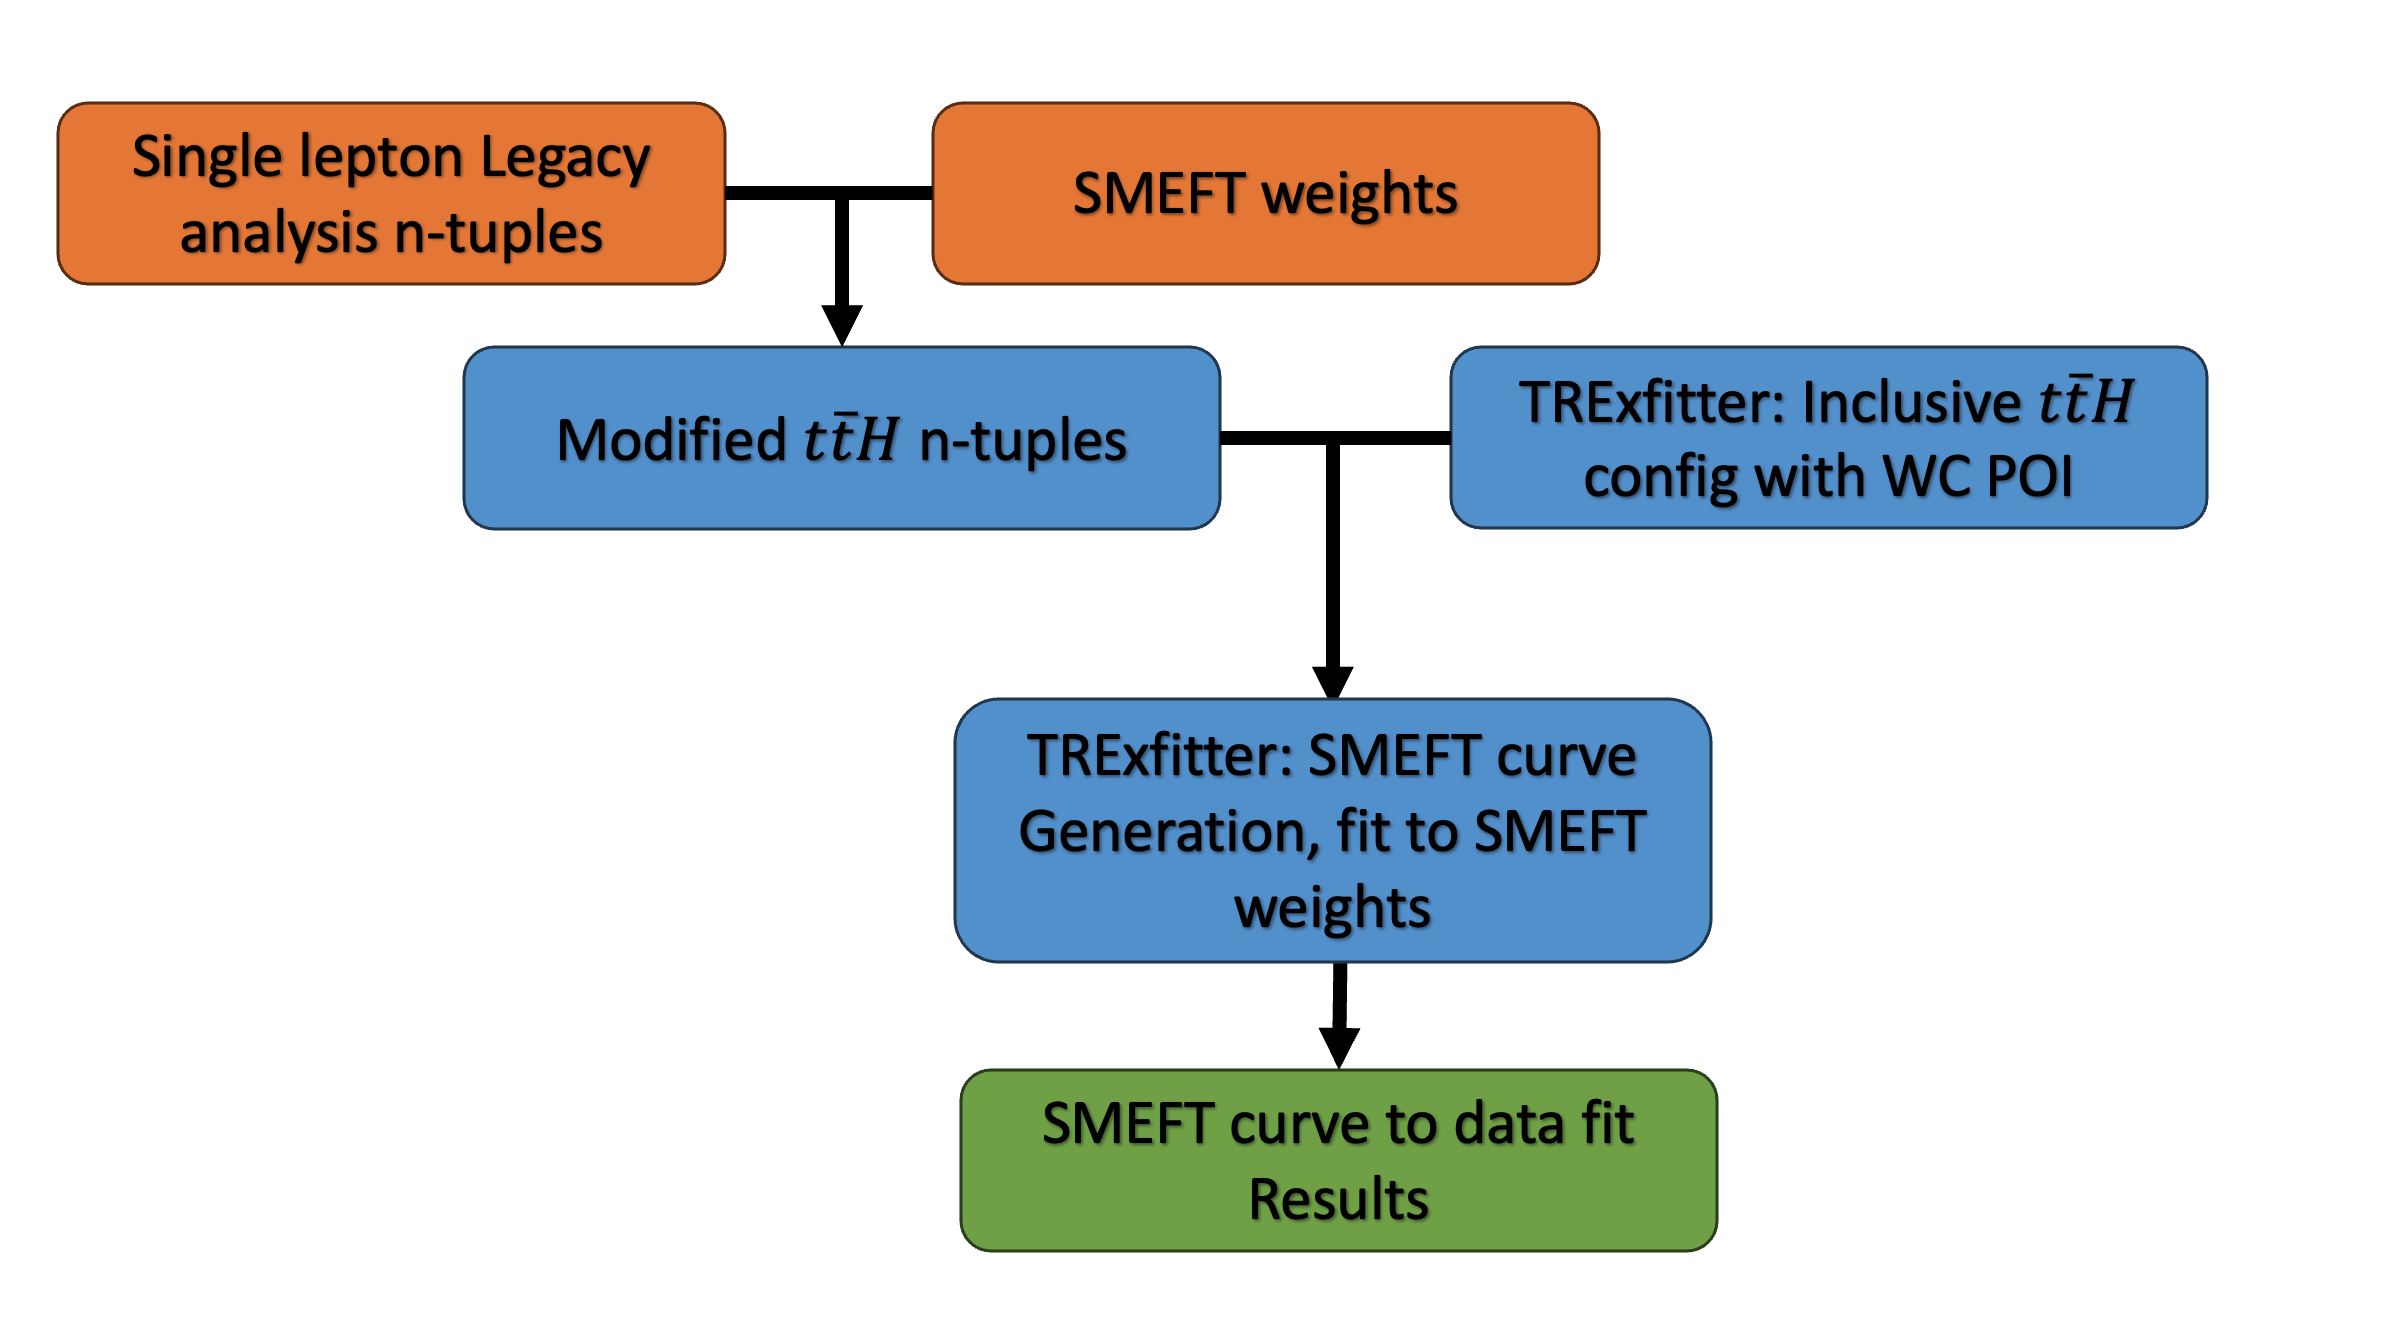
\includegraphics[width=0.7\linewidth]{Section_eft_tth/EFT_workflow.png}
    \caption{Enter Caption}
    \label{fig:EFT_workflow}
\end{figure}
\subsection{EFT Weights}
The EFT weights that we read into the SM sample are split by STXS bin and if they are linear or quadratic in nature. The linear weights only include the SM-EFT mixing contributions where as the quadratic weights include contributions from both the mixing term and pure BSM term.
\subsection{Exploiting the Higgs $p_T$ spectrum}
As the weights provided are split by STXS region, the created predictions are also split into STXS regions. Doing so reveals how each region evolves and their regime changes form being dominated by the linear coefficient to quadratic coefficient becoming more present. Thus, how different STXS regions contribute to the sensitivity of the fitted WC. Intuition would suggest that the higher STXS region EFT predictions would contain a more dominant quadratic regime and hence these regions would be a more sensitive. A quick test for this would be to remove these regions from our fit and see if the effect on the central value and precision of our fitted WC. \textcolor{red}{ask tony how many plots to show, 3 for each WC?}
\section{Results}
\subsection{$c_{\phi G}$
\subsection{$c_{tG}$}
\subsection{$c_{t\phi}$}
\subsection{Dropping STXS 5 and 6}
\subsection{Combined Results}
\section{Discussion}
